\documentclass[12pt]{article}
\usepackage[total={18cm,22cm},top=3cm,left=2cm,right=2cm]{geometry}
\parindent=0mm
\usepackage[utf8]{inputenc}

\usepackage{hyperref}

\usepackage{multicol}

\usepackage{graphicx}

\usepackage{amsmath}

\usepackage{tikz}
\usepackage{enumitem}
\definecolor{azulF}{rgb}{.0,.0,.3}
\newcommand{\cnumero}[2]{\tikz[baseline=(myanchor.base)]
\node[minimum size=0.2cm,circle,
inner sep=1pt,draw, #2, thick, fill=#2](myanchor)
{\color{white}\bfseries\fontsize{8}{8}#1};}

\newcommand*{\itembolasazules}[1]{\protect\cnumero{#1}{azulF}}

\usepackage{fancyhdr}
\pagestyle{fancy}
\fancyhf{}
%TODO
\fancyhead[L]{TEORÍA DE SISTEMAS - INVESTIGACIÓN}
%TODO
\fancyhead[R]{UNAH-VS}
\fancyfoot[C]{\thepage}

\renewcommand*\contentsname{Contenido}

\begin{document}
%*******************************************************
% Portada
%*******************************************************
\begin{titlepage}

  \begin{center}
    {\includegraphics[width=0.65\linewidth]{$HOME/Imágenes/Imgs/unahvs-logo.png}\par}
  
    {\bfseries\Huge Universidad Nacional Autónoma de\\
                     Honduras en el valle de Sula \par}
  
    \vspace{1cm}
  
%TODO
    {\scshape\huge TEORÍA DE SISTEMAS\par}
  
    \vspace{1cm}
  
%TODO
    {\scshape\Large 
      Tareas de Investigación
    }
  
    \vfill 
    {\large Catedrático:\par} %TODO
    {\large Ing. Tania Melissa Pineda Godoy\par} %TODO
  
    \vfill
    {\large Alumno: \par}
    {\large Jimmy Xavier Triminio Hernández - 20122008197 \par}

    \vfill
    {\large FEBRERO 2023\par} %TODO

  \end{center}

\end{titlepage}

%*******************************************************
% Contenido 
%*******************************************************
\newpage
\tableofcontents

%*******************************************************
% Introducción
%*******************************************************
%\newpage
\section{¿Qué es la Cadena de Valor?}

  \textit{La cadena de valor} es un modelo teórico y gráfico que permite describir las
  actividades de una organización para generar valor al cliente final y a la misma
  \textit{empresa}. Esta herramienta se utiliza para identificar las actividades clave 
  de la empresa y las relaciones entre ellas. Estas actividades se clasifican en 
  categorías como producción, marketing, distribución y servicio al cliente. La cadena 
  de valor también se puede usar para identificar oportunidades para mejorar la 
  eficiencia \footnote{\href{https://es.wikipedia.org/wiki/Cadena_de_valor}{Wikipedia|Cadena de valor}}, reducir 
  costos y aumentar los ingresos.
  
  \begin{center}
    {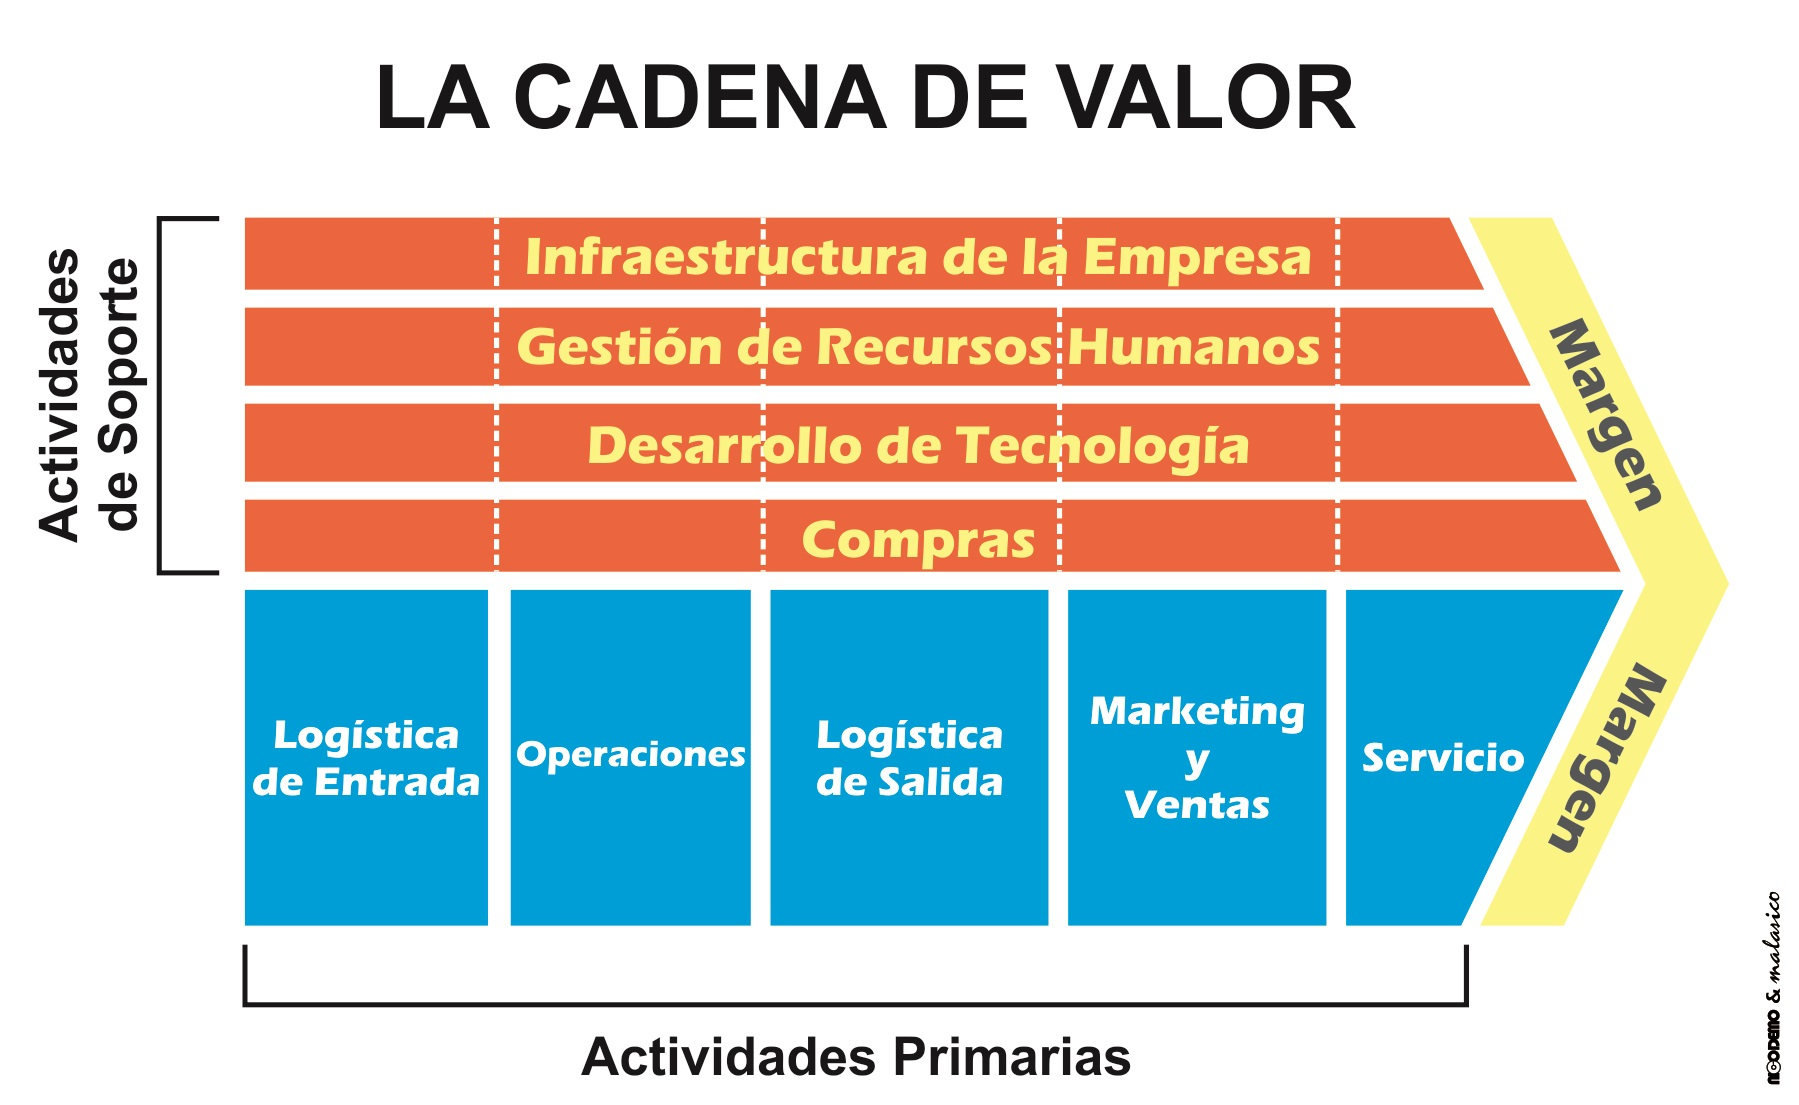
\includegraphics[width=0.75\linewidth]{Cadena_de_valor01.jpeg}\par}
  \end{center}

  \subsection{Ejemplo 1: Coca Cola}
  \textbf{Actividades primarias}\\

  Dentro de este ejemplo de la gigante de ventas, se encuentra actividades principales:
  \begin{enumerate}
    \item \textbf{Producción}: Esta empresa perfecciona su producción a través de un sistema
    de fábrica embotelladoras. Realizando concentrados de bebidas y en las plantas
    embotelladoras se hace el producto final. Coca Cola vende un 68\% de sus concentrados
    a los embotelladores.

    \item \textbf{Logística externa}: Las fábricas embotelladoras son las que distribuyen
    los productos, a través de los empleados que se encargan de distribuirlos. Algunos
    productos no son distribuidos en todos los países, esto lo decide la empresa según la 
    demanda y la disponibilidad.

    \item \textbf{Ventas y marketing}: Esta empresa es una de las más grande precursora de
    la publicidad a gran escala, y que su producto se conoce y tiene un alto porcentaje de 
    venta en todas las partes del mundo.
  \end{enumerate}

  \textbf{Actividades secundarias}\\
  En estas actividades la empresa Coca Cola resalta en innovación y descentralización:

  \begin{enumerate}
    \item \textbf{Infraestructura}: Coca Cola cuenta con una Infraestructura que permite
    realizar un estrategia multi-doméstica, basada en decisiones descentralizadas y de esa
    forma lograr enfrentar las diferencias culturales y de mercado en los distintos países.

    \item \textbf{Uso de la tecnología}: Es una bebida con características únicas que la
    diferencie del restos de los refrescos, como la línea de productos light que ganó un 
    alto nivel de mercado y muchos productos diferentes a parte del tradicional que no 
    deja del faltar.

    \item \textbf{Recursos humanos}: Coca Cola es una empresa totalmente comprometida en 
    cuanto a la capacitación de sus trabajadores, para que tenga la capacidad de elaborar
    un producto de calidad que logre satisfacer al competitivo mercado y se esfuerza para 
    que dentro de la empresa no hay ningún tipo de discriminación. 
  \end{enumerate}

  \textbf{Resultado final}\\
  El alto índice de fortalezas que comprende esta gran empresa, se identifica a través de 
  todas las ventajas que tiene a todos sus competidores, lo que le ha beneficiado en cuanto
  a su exitoso desarrollo por medio de la aplicación de sus eficientes estrategias.

  \subsection{Ejemplo 2: Empresa de Servicios (\textit{restaurantes})}
  \textbf{Actividades primarias}\\

  \begin{enumerate}
    \item \textbf{Logística interna}: se trata de la adquisición de la materia prima, como
    los ingredientes, proteínas y vegetales que se necesitan para la elaboración de las 
    comidas.

    \item \textbf{Logística externa}: esta actividad no se realiza, y que no distribuye sus
    productos externamente del restaurante, sino es comercializado para ser consumido dentro
    del lugar de ventas.

    \item \textbf{Actividad operacional}: es ejecutada por el personal que transforman todos
    los ingredientes en el plato final.

    \item \textbf{Servicio}: Esta es la actividad principal del restaurante, debido a que la recepción, los mozos y la buena atención es el servicio que recibirán los comensales.

    \item \textbf{Marketing}: es la publicidad en las redes sociales que ayudan a dar a
    conocer el restaurante.
  \end{enumerate}

  \textbf{Actividades secundarias}\\
  \begin{enumerate}
    \item \textbf{Infraestructura}: es el lugar o local donde se realiza el funcionamiento del restaurante.
    
    \item \textbf{Uso de la tecnología}: son todas aquellas maquinarias que son necesarias
    dentro de la cocina para poder ejecutar los platos finales.

    \item \textbf{Recursos humanos}: es el departamento que se encarga de realizar la
    selección de todo el personal que hará las labores de restaurante y se encarga de que
    sean capacitados.
    
    \item \textbf{Compras}: es la actividad relacionada con la compra de otros materiales
    fundamentales como las bebidas y elementos de limpieza, entre otros.
  \end{enumerate}

\section{KPI's de la unidad de tecnología de una empresa}
Los \textit{KPI's} \footnote{\textbf{KPI's}: Key Performance Indicator o Indicador Clave de Rendimiento} para el 
departamento de tecnología en una empresa, puede variar según de las misma. Algunos \textit{KPS's} comunes a todas
las empresas incluyen el costo total de la propiedad de los productos, el tiempo de respuesta y la satisfacción del
cliente. Otros \textit{KPI's} relacionadas con la tecnología pueden incluir el uso de la nube, la confiabilidad y 
la seguridad de los datos, la disponibilidad del servicio y el rendimiento continuo de toda la empresa, y los datos
y \textit{KPI's} relacionados con el desarrollo de aplicaciones.\\


\subsection{Métricas o indicadores del departamento de IT}

las categorías de KPI's que se proponen son:

\begin{enumerate}
  \item \textbf{Finanzas} la importancia alcanzada por los presupuesto de los departamentos de IT o informática, así como su importancia estratégica para el negocio, demanda que se analice y se realice un seguimiento a las inversiones y gastos realizadas en informática. El presupuesto es el instrumento de gestión por excelencia de cualquier unidad organizativa, lógicamente, eso incluye al departamento de informática o IT. Por lo que debemos en esta categoría definir (entre otros) los siguientes indicadores:
  \begin{itemize}
    \item \% del presupuesto ejecutado y no ejecutado
    \item \% gastos operativo del año
    \item \% gastos de capital del año
    \item ROI de los proyectos clave
    \item ROI ponderado del portfolio o cartera de proyectos
  \end{itemize}

  \item \textbf{Infraestructura}, el departamento de operaciones o sistemas de realizar un seguimiento al detalle de las inversiones y gastos destinados a la Infraestructura. Así mismo de la capacidad y obsolescencia tecnológico del negocio. Y ha de hacerlo por cad una de las principales áreas de negocio en donde se destinan los recursos:
  \begin{itemize}
    \item \% Infraestructura
    \item \% de inversión/gastos en Infraestructura por área de negocios: ventas, marketing, operaciones, RRHH, etc.
    \item \% de gastos en Cloud por productos y servicios
    \item \% capacidad instalada, hacerlo para aplicaciones de misión crítica para el negocio
    \item Vida útil de la Infraestructura, capacidad ociosa y nivel de madurez año o meses de la Infraestructura en general
  \end{itemize}

  \item \textbf{Calidad del servicio} medir la calidad de la gestión del departamento es de suma importancia de cara a nuestros clientes: internos y externos. Es por ello que debemos monitorear solicitudes de servicios y/o la gestión de la demanda en el departamento. En tal sentido debemos realizar un seguimiento a las operaciones.

  \begin{itemize}
    \item Cantidad de tickets recibidos
    \item \% de tickets cerrados en los períodos de tiempo
    \item \% medio de solución de los tickets
    \item \% o número de tickets resueltos por agente.
    \item Mínimamente debemos tener un control sobre la solicitudes de servicios recibidos y la respuesta promedio dada a esas solicitudes, en horas o días
    \item Evolución del blacklist o lista de tickets pendientes
  \end{itemize}

  \item \textbf{Proyectos} buena parte del presupuesto descansa en nuevas inversiones conocidas como \textit{Capex}\footnote{\textbf{Capex}: gasto de capital}. Básicamente, dichas inversiones Capex se traducen en proyectos de todo tipo y en todas las áreas. A los proyectos que son responsables del departamento de informática, es importante realizar un seguimiento de cada uno de ellos de manera individual y en su conjunto (cartera). La oficina de proyectos o PMO\footnote{\textbf{PMO}: project management office} es un excelente vehículo para ello. Muchos de los software para gestionar PMO traen su propio set de indicadores, no obstante es posible definir indicadores básicos que ayuden a conocer la salud de la cartes de proyectos en cualquier momento.

  \begin{itemize}
    \item Dashboard con una lista de todos los proyectos en desarrollo, con el nombre del proyecto,
    el jefe de proyecto.
    \item Click en el proyecto, podemos obtener un detalle del proyecto, las tareas en ejecución el \% de avance, los riesgos y los próximos entregables.
    \item \% de avance del proyecto, con indicadores de color si el proyecto está en riesgo
    \item Capacita al personal en IT
  \end{itemize}

  \item \textbf{Varios/Otros} son otras áreas en las cuales el departamento de informática pueden tener en realizar un seguimiento en detalle. Algunos indicadores potenciales son:

  \begin{itemize}
    \item \textbf{Analytics} evolución del tráfico de la página web o intranet de la empresa, Analytics de algunas web particular de la empresa, etc. Evolución de la visita a la página web, \% de incremento/descuento, ídem por páginas más visitadas.

    \item \textbf{CRM}\footnote{\textbf{CRM}: Customer Relationship Management} Analytics del CRM de la empresa, con indicadores tales como evolución de Leads, cierres de oportunidades, estadísticas por agente o vendedor, etc.

    \item \textbf{VPN}\footnote{\textbf{VPN}: son las siglas para Virtual Private Network} evolución de accesos a la red. 

    \item \textbf{HHRR} el \textit{headcount} es otra métrica de importancia para muchos departamentos IT. Personal propio vrs contratado, gasto vario por empleado (viajes, dietas, etc), gastos por comercial o vendedor, horas por proyectos y sus respectivos gastos, entre otros.

    \item \textbf{Teletrabajo} las plataformas web como Zoom y MS Teams proporcionan KPI's de interés que nos muestran, números de salas utilizadas por unidad de tiempo, tiempo de conexión de cada persona por unidad de tiempo, etc. Así mismo, es interesantes, chequear las aplicaciones del negocio más utilizadas por los teletrabajadores.
  \end{itemize}

\end{enumerate}

\section{UML}

El UML\footnote{\textbf{UML}: Lenguaje  Unificado de Modelado} son un conjunto de símbolos gráficos que se utilizan para representar los procesos y estructuras de un sistema. Los diagramas de UML más comunes son: 
\begin{itemize}
  \item Diagramas de culturales
  \item Diagramas de objetos
  \item Diagramas de secuencia
  \item diagramas de actividades
  \item Diagramas de interacción
  \item Diagramas de estado
  \item Diagramas de componentes
  \item Diagramas de despliegue
\end{itemize}
Por ejemplo, un diagrama de clase muestra la estructura de un sistema, con las clases y sus relaciones, mientras que un diagrama de secuencias muestra la secuencia de mensajes entre los objetos de un sistema.

\section{Just In Time}
\textit{Just in Time} es una técnica de fabricación usada en informática para reducir los tiempos de espera y los costos de producción, al tiempo de mejorar la calidad de los productos. Esta técnica se basa en la entrega de materiales y componentes de informática en el momento exacto en que necesiten para la producción, eliminando los tiempos de esperar en la cadena de producción. Estos significa que los componentes se producen y se entregan justo antes de que necesiten, reduciendo los costos de almacenamiento y los riesgos de obsolescencia. Además, también mejora la calidad de los productos de informática, y que cada componente se prueba antes de ser utilizado en el proceso de producción.

\section{Punto de Re-orden}
El \textbf{Punto de Re-orden}\textit{(Reorder Point)} es una herramienta de gestión de inventarios que permiten determinar el nivel de inventario óptimo para un producto. Esto significa que el punto de re-orden es el nivel de inventario en que se producirán un pedido para abastecer el inventario. El puntos de re-orden suele calcularse utilizando la fórmula de re-orden, que considera el nivel de inventario actual, el costo de pedido, el tiempo de entrega, el costo de almacenamiento y el nivel de demanda. Esta herramienta permite a la empresa reducir los costo de almacenamiento, evitando los costos de mantenimiento de inventario excesivo, y evitar los costos de mantenimiento de inventario insuficiente.

\section{La cadena de suministro}
La cadena de suministros es el conjunto de actividades, instalaciones y medios de distribución necesarias para llevar a cabo el proceso de venta de un producto o servicio desde el punto de origen de destino. Estas actividades incluyen la fabricación, el almacenamiento, el transporte, la distribución, la promoción, la entrega y, en algunos casos, la recolección. El conjunto principal de la cadena de suministro es logar un flujo de producción eficiente, económico y de la calidad pasa satisfacer las necesidades del cliente.

\newpage
\section{Bibliografía}

\begin{enumerate}
  \item \textbf{Indicadores de IT}\\ 
        \href{https://www.sydle.com/es/blog/indicadores-de-ti-605a2bd0b7cdda685648b68a}{www.sydle.com}

  \item \textbf{Indicadores para una efectiva gestión de departamento de informática}\\
        \href{https://www.itmadrid.com/5-indicadores-o-kpi-clave-para-una-efectiva-gestion-de-los-departamentos-tic-o-informatica/}{www.itmadrid.com/digital-school}

  \item \textbf{Estudio para la Optimización de la gestión de Producción}\\
        \href{https://dspace.ups.edu.ec/bitstream/123456789/5387/1/UPS-GT000505.pdf}{dspace.ups.edu.ec}

  \item \textbf{Propuesta para la profesionalización del almacenamiento y logística de una PyMe}\\ 
        Página 49\\
        \href{https://static1.squarespace.com/static/55564587e4b0d1d3fb1eda6b/t/5e29ce73907bc30696980607/1579798160559/Tomo+06+-+Memorias+Congreso+Academia+Journals+Celaya+2019.pdf}{Static.squarespace.com}
  
  \item \textbf{Cadena de suministro}\\
        \href{https://economipedia.com/definiciones/cadena-de-suministro.html}{economipedia.com}

\end{enumerate}


\end{document}

